\documentclass[serif]{beamer}

% ---------------------------------------------------------

\usepackage[utf8]{inputenc}
\usepackage[T1]{fontenc}
\usepackage[english]{babel}

% ---------------------------------------------------------

\usepackage{appendixnumberbeamer}

\setbeamertemplate{navigation symbols}{}

\addtobeamertemplate{footline}{%
	\hspace*{\fill}%
	\llap{%
		\insertframenumber\,/\,\inserttotalframenumber%
		\hspace{5pt}%
	}
	\vskip4pt%
}

% ---------------------------------------------------------

\usepackage{xcolor}
\usepackage{xspace} % \xspace

\usepackage{graphicx}

\usepackage{stackrel} % \stackrel

\usepackage{fancyvrb} % Verbatim

\usepackage{dashbox} % \dbox

\usepackage{tikz}
\usetikzlibrary{
	decorations.pathreplacing,
	positioning
}

\usepackage{pifont} % \ding

% ---------------------------------------------------------

\usepackage{amsmath} % align*

\usepackage{amssymb} % \mathbb
\usepackage{mathrsfs} % \mathscr
\usepackage{bbm} % \mathbbm
\usepackage{tensor} % \tensor

\usepackage{mathabx} % \ast, \bigast

\usepackage{mathpartir}

\let\oldexists\exists
\let\exists\relax\DeclareMathOperator{\exists}{\oldexists}
\let\oldforall\forall
\let\forall\relax\DeclareMathOperator{\forall}{\oldforall}

\DeclareMathOperator{\lambdaabs}{\lambda}
\DeclareMathOperator{\muabs}{\mu}
\DeclareMathOperator{\nuabs}{\nu}

% ---------------------------------------------------------

\usepackage{listings}
\usepackage{lstcaml}

% ---------------------------------------------------------

\usepackage{overtools}

% ---------------------------------------------------------

\newcommand{\mathhyphen}{{\hbox{-}}}

\newcommand{\eqdef}{\stackrel{\Delta}=}

\newcommand\doubleplus{+\kern-1.3ex+\kern0.8ex}
\newcommand\mdoubleplus{\ensuremath{\mathbin{+\mkern-10mu+}}}

\newcommand{\sref}[1]{\S\ref{#1}}
\newcommand{\fref}[1]{Figure~\ref{#1}}

\newcommand{\OCaml}{\textsc{OCaml}\xspace}
\newcommand{\Coq}{\textsc{Coq}\xspace}
\newcommand{\Iris}{\textsc{Iris}\xspace}

\newcommand{\triple}[3]{%
	\left\lbrace\, #1 \,\right\rbrace\ %
	#2\ %
	\left\lbrace\, #3 \,\right\rbrace%
}
\newcommand{\triplePretty}[3]{%
	\begin{array}{c}
			\left\lbrace\, #1 \,\right\rbrace
		\\ \hline
			#2
		\\ \hline
			\left\lbrace\, #3 \,\right\rbrace
	\end{array}
}
\newcommand{\atriple}[6]{%
	\left\langle\, \forall #1 \cdot\, #2 \,\right\rangle\ %
	#3\ %
	\left\langle\, #4 \cdot\, \lambda\, \exists #5 \cdot\, #6 \,\right\rangle%
}
\newcommand{\atriplePretty}[6]{%
	\begin{array}{c}
			\left\langle\, \forall #1 \cdot\, #2 \,\right\rangle
		\\ \hline
			#3
		\\ \hline
			\left\langle\, \exists #4 \cdot\, \lambda\, #5 \cdot\, #6 \,\right\rangle
	\end{array}
}
\newcommand{\atripleExt}[9]{%
	\left\lbrace\, #1 \,\right\rbrace\ %
	\left\langle\, \forall #2 \cdot\, #3 \,\right\rangle\ %
	#4,\ #5\ %
	\left\langle\, \exists #6 \cdot\, #7 \,\right\rangle\ %
	\left\lbrace\, \lambda\, #8 \cdot\, #9 \,\right\rbrace%
}
\newcommand{\atripleExtPretty}[9]{%
	\begin{array}{c}
			\left\lbrace\, #1 \,\right\rbrace
		\\ \hline
			\left\langle\, \forall #2 \cdot\, #3 \,\right\rangle
		\\ \hline
			#4,\ #5
		\\ \hline
			\left\langle\, \exists #6 \cdot\, #7 \,\right\rangle
		\\ \hline
			\left\lbrace\, \lambda\, #8 \cdot\, #9 \,\right\rbrace
	\end{array}
}

\newcommand{\term}[1]{\texttt{#1}}
\newcommand{\nterm}[1]{\mathrm{#1}}

\newcommand{\exprUnit}{\term{(}\term{)}}
\newcommand{\exprRef}[1]{\term{ref}\ #1}
\newcommand{\exprSeq}[2]{#1\,\term{;}\,#2}
\newcommand{\exprIf}[3]{\term{if}\ #1\ \term{then}\ #2\ \term{else}\ #3}
\newcommand{\exprLoad}[1]{!\,#1}
\newcommand{\exprStore}[2]{#1\leftarrow#2}
\newcommand{\exprCall}[2]{#1\ #2}
\newcommand{\exprNone}{\term{NONE}}
\newcommand{\exprSome}[1]{\term{SOME}\ #1}

\newcommand{\iEmpty}{\emptyset}
\newcommand{\iTrue}{\mathrm{True}}
\newcommand{\iFalse}{\mathrm{False}}
\newcommand{\iSep}{\ast}
\newcommand{\iBigsep}{\bigast}
\newcommand{\iSepimp}{\mathrel{-\mkern-6mu\sep}}
\newcommand{\iBupd}{|\!\!\!\Rrightarrow}
\newcommand{\iPers}{\square}
\newcommand{\iAuth}[1]{\bullet\,#1}
\newcommand{\iFrag}[1]{\circ\,#1}
\newcommand{\iGhost}[2]{\dbox{\strut\ensuremath{#2}}^{#1}}
\newcommand{\iInv}[2]{\boxed{\strut\ensuremath{#2}}^{#1}}


% ---------------------------------------------------------

\title{
	Verification of Chase-Lev work-stealing deque
}
\author{
	Clément Allain \\
	François Pottier
}

% ---------------------------------------------------------
% ---------------------------------------------------------

\begin{document}

% ---------------------------------------------------------

\begin{frame}
\titlepage
\end{frame}

% ---------------------------------------------------------

\begin{frame}[fragile]{Verification of a scheduler}
%\begin{itemize}
%	\item domainslib (\OCaml~5)
%	\item Taskflow (C++)
%\end{itemize}
%\vfill
\begin{Verbatim}[commandchars=\\\{\}]
let rec fib pool n =
  if n < 2 then 1 else
  let r1 = \textcolor{blue}{async} pool (fun () -> fib_par (n - 1)) in
  let r2 = \textcolor{blue}{async} pool (fun () -> fib_par (n - 2)) in
  \textcolor{blue}{await} pool r1 + \textcolor{blue}{await} pool r2
\end{Verbatim}
\end{frame}
\begin{frame}{Work-stealing}
\centering
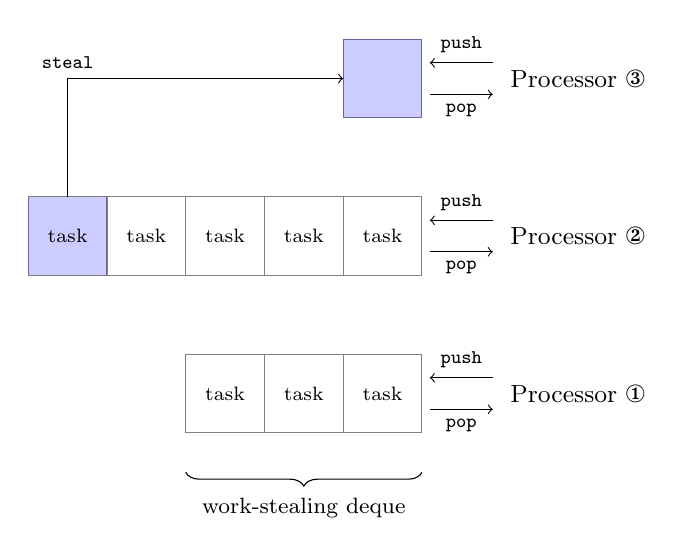
\begin{tikzpicture}
	\def\sep{1}
	\def\hsep{0.1}
	\def\vsep{0.3}
	\def\lenI{3}
	\def\lenxI{0}
	\def\lenII{4}
	\def\lenxII{1}
	\def\lenIII{0}
	\def\lenxIII{1}
	
	\node[right] at (1, 0.5) {\small Processor \ding{172}} ;
	\draw[step=1cm, gray] (0, 0) grid ++(-\lenI, 1) ;
	\draw[step=1cm, gray] (-\lenI, 0) grid ++(-\lenxI, 1) ;
	\fill[blue, opacity=0.2] (-\lenI, 0) rectangle ++(-\lenxI, 1) ;
	\draw[decorate, decoration={brace, amplitude=5pt}] (0, -0.5) -- ++(-\lenI, 0) node [midway, below, yshift=-2mm] {\footnotesize work-stealing deque} ;
	\draw[->] (\hsep, \vsep) -- ++(1 - 2 * \hsep, 0) node[midway, below] {\scriptsize\texttt{pop}} ;
	\draw[->] (1 - \hsep, 1 - \vsep) -- ++(2 * \hsep - 1, 0) node[midway, above] {\scriptsize\texttt{push}} ;
	\foreach \x in {1, ..., \lenI} {
		\node at (0.5 - \x, 0.5) {\scriptsize task} ;
	}
	
	\node[right] at (1, \sep + 1.5) {\small Processor \ding{173}} ;
	\draw[step=1cm, gray] (0, \sep + 1) grid ++(-\lenII, 1) ;
	\draw[step=1cm, gray] (-\lenII, \sep + 1) grid ++(-\lenxII, 1) ;
	\fill[blue, opacity=0.2] (-\lenII, \sep + 1) rectangle ++(-\lenxII, 1) ;
	\draw[->] (\hsep, \sep + 1 + \vsep) -- ++(1 - 2 * \hsep, 0) node[midway, below] {\scriptsize\texttt{pop}} ;
	\draw[->] (1 - \hsep, \sep + 2 - \vsep) -- ++(2 * \hsep - 1, 0) node[midway, above] {\scriptsize\texttt{push}} ;
	\foreach \x in {1, ..., \lenII} {
		\node at (0.5 - \x, \sep + 1.5) {\scriptsize task} ;
	}
	\node at (0.5 - \lenII - \lenxII, \sep + 1.5) {\scriptsize task} ;
	
	\node[right] at (1, 2 * \sep + 2.5) {\small Processor \ding{174}} ;
	\draw[step=1cm, gray] (0, 2 * \sep + 2) grid ++(-\lenIII, 1) ;
	\draw[step=1cm, gray] (-\lenIII, 2 * \sep + 2) grid ++(-\lenxIII, 1) ;
	\fill[blue, opacity=0.2] (-\lenIII, 2 * \sep + 2) rectangle ++(-\lenxIII, 1) ;
	\draw[->] (\hsep, 2 * \sep + 2 + \vsep) -- ++(1 - 2 * \hsep, 0) node[midway, below] {\scriptsize\texttt{pop}} ;
	\draw[->] (1 - \hsep, 2 * \sep + 3 - \vsep) -- ++(2 * \hsep - 1, 0) node[midway, above] {\scriptsize\texttt{push}} ;
	
	\draw[->, to path={|- node[above] {\scriptsize\texttt{steal}} (\tikztotarget)}] (0.5 - \lenII - \lenxII, \sep + 2) to (- \lenIII - \lenxIII, 2 * \sep + 2.5) ;
\end{tikzpicture}
\end{frame}

% ---------------------------------------------------------

\begin{frame}{Chase-Lev work-stealing deque}
\begin{enumerate}
	\item
		\textit{The Implementation of the Cilk-5 Multithreaded Language}. \\
		Frigo, Leiserson \& Randall (1998).
		\begin{itemize}
			\item lock
		\end{itemize}
	\item
		\textit{Thread Scheduling for Multiprogrammed Multiprocessors}. \\
		Arora, Blumofe \& Plaxton (1998).
		\begin{itemize}
			\item non-blocking
			\item one fixed size array, potential overflow
		\end{itemize}
	\item
		\textit{A dynamic-sized nonblocking work stealing deque}. \\
		Hendler, Lev, Moir, \& Shavit (2004).
		\begin{itemize}
			\item non-blocking
			\item list of small arrays, no overflow
		\end{itemize}
	\item
		\underline{\textit{Dynamic circular work-stealing deque}}. \\
		Chase \& Lev (2005).
		\begin{itemize}
			\item non-blocking
			\item circular arrays, no overflow
		\end{itemize}
\end{enumerate}
\end{frame}
\begin{frame}{Why is it interesting?}
\begin{itemize}
	\setlength\itemsep{1em}
	\item Demonstration of Iris on a (simplified) real-life concurrent data structure.
	\item Rich ghost state to enforce a subtle protocol.
		\begin{itemize}
			\item logical state $\neq$ physical state
			\item external future-dependent linearization point
		\end{itemize}
	\item Nontrivial use of prophecy variables.
\end{itemize}
\end{frame}

\begin{frame}{The rest of this talk}
\begin{itemize}
	\item Specification using logically atomic triples.
	\item Rough idea of how the data structure works.
	\item Why we need prophecy variables.
\end{itemize}
\end{frame}
\section{Specification}

\begin{frame}{Specification --- \texttt{chaselev\_make}}
\small
\centering
\[
	\triplePretty{
		\iTrue
	}{
		\texttt{chaselev\_make}\ \exprUnit
	}{
		\lambda\ t \ldotp
		\tikz[baseline, remember picture]{\node[anchor=base] (inv_1) {${
			\textcolor{blue}{\mathrm{chaselev \mathhyphen inv}\ t\ \iota}
		}$}} \iSep
		\tikz[baseline, remember picture]{\node[anchor=base] (model_1) {${
			\textcolor{red}{\mathrm{chaselev \mathhyphen model}\ t\ []}
		}$}} \iSep
		\tikz[baseline, remember picture]{\node[anchor=base] (owner_1) {${
			\textcolor{teal}{\mathrm{chaselev \mathhyphen owner}\ t}
		}$}}
	}
\]
\vfill
\only<2>{
	\tikz[remember picture] \node[align=left] (inv_2) {
		$t$ is an instance of Chase-Lev deque. \\
		Enforces a protocol (using an Iris invariant).
	} ;
	\begin{tikzpicture}[remember picture, overlay]
		\path[draw=blue, thick, ->] (inv_2.north) to [out=100, in=-100] (inv_1.south) ;
	\end{tikzpicture}
}
\only<3>{
	\tikz[remember picture] \node[align=left] (model_2) {
		Asserts the list of values that $t$ logically contains.
	} ;
	\begin{tikzpicture}[remember picture, overlay]
		\path[draw=red, thick, ->] (model_2.north) to [out=100, in=-100] (model_1.south) ;
	\end{tikzpicture}
}
\only<4>{
	\tikz[remember picture] \node[align=left] (owner_2) {
		Gives the owner exclusive access to his end of $t$.
	} ;
	\begin{tikzpicture}[remember picture, overlay]
		\path[draw=teal, thick, ->] (owner_2.north) to [out=100, in=-100] (owner_1.south) ;
	\end{tikzpicture}
}
\end{frame}

% ---------------------------------------------------------

\begin{frame}{Specification --- \texttt{chaselev\_push}}
\centering
\[
	\atripleExtPretty{
		\tikz[baseline, remember picture]{\node[anchor=base] (inv_1) {${
			\textcolor{blue}{\mathrm{chaselev \mathhyphen inv}\ t\ \iota}
		}$}} \iSep
		\tikz[baseline, remember picture]{\node[anchor=base] (owner_1) {${
			\textcolor{red}{\mathrm{chaselev \mathhyphen owner}\ t}
		}$}}
	}{
		\mathit{vs}
	}{
		\tikz[baseline, remember picture]{\node[anchor=base] (model_1) {${
			\textcolor{teal}{\mathrm{chaselev \mathhyphen model}\ t\ \mathit{vs}}
		}$}}
	}{
		\texttt{chaselev\_push}\ t\ v
	}{
		\uparrow\iota
	}{
	}{
		\tikz[baseline, remember picture]{\node[anchor=base] (model_2) {${
			\textcolor{teal}{\mathrm{chaselev \mathhyphen model}\ t\ (\mathit{vs} \mdoubleplus [v])}
		}$}}
	}{
		\exprUnit
	}{
		\tikz[baseline, remember picture]{\node[anchor=base] (owner_2) {${
			\textcolor{red}{\mathrm{chaselev \mathhyphen owner}\ t}
		}$}}
	}
\]
\begin{overbox}<2>
	\small
	\centering
	Specification of a concurrent operation ($\simeq$ transaction):
	
	standard triple + logically atomic triple
	
	\[
		\atripleExtPretty{
			\textcolor{red}{P}
		}{
			\textcolor{purple}{\overline{x}}
		}{
			\textcolor{teal}{P_\mathrm{lin}}
		}{
			e
		}{
			\mathcal{E}
		}{
			\textcolor{purple}{\overline{y}}
		}{
			\textcolor{teal}{Q_\mathrm{lin}}
		}{
			res
		}{
			\textcolor{red}{Q}
		}
	\]
	\begin{align*}
			\textcolor{red}{P}
			&:
			\text{private precondition}
		\\
			\textcolor{red}{Q}
			&:
			\text{private postcondition}
		\\
			\textcolor{teal}{P_\mathrm{lin}}
			&:
			\text{public precondition}
		\\
			\textcolor{teal}{Q_\mathrm{lin}}
			&:
			\text{public postcondition}
	\end{align*}
\end{overbox}
\begin{overbox}<3>
	For a concurrent data structure:
	
	\[
		\atripleExtPretty{
			\textcolor{blue}{\mathrm{??? \mathhyphen inv} \cdots} \iSep
			\textcolor{red}{P}
		}{
			\textcolor{purple}{\overline{x}}
		}{
			\textcolor{teal}{\mathrm{??? \mathhyphen model} \cdots}
		}{
			e
		}{
			\mathcal{E}
		}{
			\textcolor{purple}{\overline{y}}
		}{
			\textcolor{teal}{\mathrm{??? \mathhyphen model} \cdots}
		}{
			res
		}{
			\textcolor{red}{Q}
		}
	\]
\end{overbox}
\vfill
\only<4>{
	\tikz[remember picture] \node[align=left] (inv_2) {
		$t$ is an instance of Chase-Lev deque.
	} ;
	\begin{tikzpicture}[remember picture, overlay]
		\path[draw=blue, thick, ->] (inv_2.north) to [out=100, in=-100] (inv_1.south) ;
	\end{tikzpicture}
}
\only<5>{
	\tikz[remember picture] \node[align=left] (owner_3) {
		This operation is reserved to the owner of $t$.
	} ;
	\begin{tikzpicture}[remember picture, overlay]
		\path[draw=red, thick, ->] (owner_3.north) to [out=100, in=-100] (owner_1.south) ;
		\path[draw=red, thick, ->] (owner_3.north) to [out=100, in=-100] ([xshift=5mm]owner_2.south) ;
	\end{tikzpicture}
}
\only<6>{
	\tikz[remember picture] \node[align=left] (model_3) {
		$v$ is atomically pushed at the owner's end of $t$.
	} ;
	\begin{tikzpicture}[remember picture, overlay]
		\path[draw=teal, thick, ->] (model_3.north) to [out=100, in=-100] (model_1.south) ;
		\path[draw=teal, thick, ->] (model_3.north) to [out=100, in=-100] ([xshift=1cm]model_2.south) ;
	\end{tikzpicture}
}
\end{frame}

% ---------------------------------------------------------

\begin{frame}{Specification --- \texttt{chaselev\_pop}}
\footnotesize
\centering
\[
	\atripleExtPretty{
		\tikz[baseline, remember picture]{\node[anchor=base] (inv_1) {${
			\textcolor{blue}{\mathrm{chaselev \mathhyphen inv}\ t\ \iota}
		}$}} \iSep
		\tikz[baseline, remember picture]{\node[anchor=base] (owner_1) {${
			\textcolor{red}{\mathrm{chaselev \mathhyphen owner}\ t}
		}$}}
	}{
		\mathit{vs}
	}{
		\tikz[baseline, remember picture]{\node[anchor=base] (model_1) {${
			\textcolor{teal}{\mathrm{chaselev \mathhyphen model}\ t\ \mathit{vs}}
		}$}}
	}{
		\texttt{chaselev\_pop}\ t
	}{
		\uparrow\iota
	}{
		o
	}{
		\tikz[baseline, remember picture]{\node[anchor=base] (model_2) {${
			\textcolor{teal}{
				\bigvee\left[\begin{array}{l}
						\mathit{vs} = [] \iSep
						o = \exprNone \iSep
						\textcolor{teal}{\mathrm{chaselev \mathhyphen model}\ t\ []}
					\\
						\exists v, \mathit{vs'} \ldotp
						\mathit{vs} = \mathit{vs'} \mdoubleplus [v] \iSep
						o = \exprSome{v} \iSep
						\textcolor{teal}{\mathrm{chaselev \mathhyphen model}\ t\ \mathit{vs'}}
				\end{array}\right]
			}
		}$}}
	}{
		o
	}{
		\tikz[baseline, remember picture]{\node[anchor=base] (owner_2) {${
			\textcolor{red}{\mathrm{chaselev \mathhyphen owner}\ t}
		}$}}
	}
\]
\vfill
\only<2>{
	\tikz[remember picture] \node[align=left] (inv_2) {
		$t$ is an instance of Chase-Lev deque.
	} ;
	\begin{tikzpicture}[remember picture, overlay]
		\path[draw=blue, thick, ->] (inv_2.north) to [out=100, in=-100] (inv_1.south) ;
	\end{tikzpicture}
}
\only<3>{
	\tikz[remember picture] \node[align=left] (owner_3) {
		This operation is reserved to the owner of $t$.
	} ;
	\begin{tikzpicture}[remember picture, overlay]
		\path[draw=red, thick, ->] (owner_3.north) to [out=100, in=-100] (owner_1.south) ;
		\path[draw=red, thick, ->] (owner_3.north) to [out=100, in=-100] ([xshift=5mm]owner_2.south) ;
	\end{tikzpicture}
}
\only<4>{
	\tikz[remember picture] \node[align=left] (model_3) {
		Either 1) $t$ is seen empty \\
		or 2) some value $v$ is atomically popped at the owner's end of $t$.
	} ;
	\begin{tikzpicture}[remember picture, overlay]
		\path[draw=teal, thick, ->] (model_3.north) to [out=100, in=-100] (model_1.south) ;
		\path[draw=teal, thick, ->] (model_3.north) to [out=100, in=-100] ([xshift=1cm]model_2.south) ;
	\end{tikzpicture}
}
\end{frame}

% ---------------------------------------------------------

\begin{frame}{Specification --- \texttt{chaselev\_steal}}
\footnotesize
\centering
\[
	\atripleExtPretty{
		\tikz[baseline, remember picture]{\node[anchor=base] (inv_1) {${
			\textcolor{blue}{\mathrm{chaselev \mathhyphen inv}\ t\ \iota}
		}$}}
	}{
		\mathit{vs}
	}{
		\tikz[baseline, remember picture]{\node[anchor=base] (model_1) {${
			\textcolor{teal}{\mathrm{chaselev \mathhyphen model}\ t\ \mathit{vs}}
		}$}}
	}{
		\texttt{chaselev\_steal}\ t
	}{
		\uparrow\iota
	}{
		o
	}{
		\tikz[baseline, remember picture]{\node[anchor=base] (model_2) {${
			\textcolor{teal}{
				\bigvee\left[\begin{array}{l}
						\mathit{vs} = [] \iSep
						o = \exprNone \iSep
						\mathrm{chaselev \mathhyphen model}\ t\ []
					\\
						\exists v, \mathit{vs'} \ldotp
						\mathit{vs} = v :: \mathit{vs'} \iSep
						o = \exprSome{v} \iSep
						\mathrm{chaselev \mathhyphen model}\ t\ \mathit{vs'}
				\end{array}\right]
			}
		}$}}
	}{
		o
	}{
		\iTrue
	}
\]
\vfill
\only<2>{
	\tikz[remember picture] \node[align=left] (inv_2) {
		$t$ is an instance of Chase-Lev deque.
	} ;
	\begin{tikzpicture}[remember picture, overlay]
		\path[draw=blue, thick, ->] (inv_2.north) to [out=100, in=-100] (inv_1.south) ;
	\end{tikzpicture}
}
\only<3>{
	\tikz[remember picture] \node[align=left] (model_3) {
		Either 1) $t$ is seen empty \\
		or 2) some value $v$ is atomically popped at the thieves' end of $t$.
	} ;
	\begin{tikzpicture}[remember picture, overlay]
		\path[draw=teal, thick, ->] (model_3.north) to [out=100, in=-100] (model_1.south) ;
		\path[draw=teal, thick, ->] (model_3.north) to [out=100, in=-100] ([xshift=1cm]model_2.south) ;
	\end{tikzpicture}
}
\end{frame}
\begin{frame}{Physical state}
\centering
\hspace{-1cm}
\begin{tikzpicture}[scale=1.15]
	\def\hist{2}
	\def\histext{1}
	\def\pub{3}
	\def\priv{2.8}
	
	\only<1->{
		\draw[step=1cm, gray, thin] (0, 0) grid (\hist + \pub + \priv, 1) ;
		\draw[decorate, decoration={brace, amplitude=5pt}] (-0.2, 0) -- (-0.2, 1) node [midway, xshift=-7mm] {data} ;
	}
	
	\only<2->{
		\draw[very thick] (\hist, 0) -- (\hist, 1) node[label=above:front] {} ;
	}
	
	\only<4->{
		\draw[very thick] (\hist + \pub, 0) -- (\hist + \pub, 1) node[label=above:back] {} ;
	}
	
	\only<5->{
		\fill[red, opacity=0.2] (\hist + \pub, 0) rectangle (\hist + \pub + \priv, 1) ;
		\draw[decorate, decoration={brace, amplitude=5pt}] (\hist + \pub + \priv, -0.2) -- (\hist + \pub, -0.2) node [midway, yshift=-5mm] {priv} ;
	}
	
	\only<6->{
		\fill[green, opacity=0.2] (\hist, 0) rectangle (\hist + \pub, 1) ;
		\draw[decorate, decoration={brace, amplitude=5pt}] (\hist + \pub, -0.2) -- (\hist, -0.2) node [midway, yshift=-5mm] {pub} ;
	}
	\only<7->{
		\fill[blue, opacity=0.2] (0,0) rectangle (\hist, 1) ;
		\draw[decorate, decoration={brace, amplitude=5pt}] (\hist, -0.2) -- (0, -0.2) node [midway, yshift=-5mm] {hist} ;
	}
		
	\only<9->{
		\fill[blue, opacity=0.2] (\hist,0) rectangle (\hist + \histext, 1) ;
		\draw[decorate, decoration={brace, amplitude=5pt}] (\hist + \histext, -1) -- (0, -1) node [midway, yshift=-5mm] {hist\textsubscript{+}} ;
	}
	
	\only<10->{
		\draw[thick, ->, blue] (\hist, 0.5) -- (\hist + 1, 0.5) node[label=below left:{\footnotesize\texttt{steal}}] {} ;
		\draw[thick, ->, teal] (\hist + \pub, 0.5) -- (\hist + \pub - 1, 0.5) node[label=below right:{\footnotesize\texttt{pop}}] {} ;
		\draw[thick, ->, red] (\hist + \pub, 0.5) -- (\hist + \pub + 1, 0.5) node[label=below left:{\footnotesize\texttt{push}}] {} ;
	}
\end{tikzpicture}
\vfill
\begin{itemize}
	\item[data:]<1-> infinite array storing all values
	\item[front:]<2-> \emph{monotone} index for thieves' end
	\item[back:]<4-> index for owner's end
\end{itemize}
\begin{itemize}
	\item[priv:]<5-> list of private values (controlled by owner)
	\item[pub:]<6-> list of public values (= model)
	\item[hist:]<7-> \emph{monotone} list of history values
	\item[hist\textsubscript{+}:]<9-> \emph{monotone} list of extended history values
\end{itemize}
\begin{overbox}<3>
	\begin{mathpar}
		\inferrule*[lab=ChaselevFrontValid]
			{
				\iGhost{\gamma\mathrm{.front}}{\iAuth{front_1}}
			\and
				\iGhost{\gamma\mathrm{.front}}{\iFrag{front_2}}
			}{
				front2 \leq front1
			}
		\and
		\inferrule*[lab=ChaselevFrontUpdate]
			{
				front \leq front'
			\and
				\iGhost{\gamma\mathrm{.front}}{\iAuth{front}}
			}{
				\iGhost{\gamma\mathrm{.front}}{\iAuth{front'}}
			}
		\and
		\inferrule*[lab=ChaselevFrontFragGet]
			{
				\iGhost{\gamma\mathrm{.front}}{\iAuth{front}}
			}{
				\iGhost{\gamma\mathrm{.front}}{\iFrag{front}}
			}
	\end{mathpar}
\end{overbox}
\begin{overbox}<8>
	\begin{mathpar}
		\inferrule*[lab=ChaselevHistValid]
			{
				\iGhost{\gamma\mathrm{.hist}}{\iAuth{hist_1}}
			\and
				\iGhost{\gamma\mathrm{.hist}}{\iFrag{hist_2}}
			}{
				hist_2 \sqsubseteq_\mathrm{prefix} hist_1
			}
		\and
		\inferrule*[lab=ChaselevHistUpdate]
			{
				\iGhost{\gamma\mathrm{.hist}}{\iAuth{hist}}
			}{
				\iGhost{\gamma\mathrm{.hist}}{\iAuth{(hist \mdoubleplus [v])}}
			}
		\and
		\inferrule*[lab=ChaselevHistFragGet]
			{
				\iGhost{\gamma\mathrm{.hist}}{\iAuth{hist}}
			}{
				\iGhost{\gamma\mathrm{.hist}}{\iFrag{hist}}
			}
	\end{mathpar}
\end{overbox}
\end{frame}

% ---------------------------------------------------------

\begin{frame}{Logical state}
\centering
\begin{tikzpicture}
	\def\width{4cm}
	\def\height{2cm}
	
	\only<1->{
		\node[align=center] (s1) {
			\ding{172} empty \\
			\begin{tikzpicture}[scale=0.5]
				\def\hist{2}
				\def\priv{2.8}
		
				\draw[step=1cm, gray, thin] (0, 0) grid (\hist + \priv, 1) ;
				
				\fill[blue, opacity=0.2] (0, 0) rectangle (\hist, 1) ;
				\draw[very thick] (\hist, 1) -- (\hist, 0) node[yshift=2mm, label=below:{\tiny front = back}] {} ;
				\fill[red, opacity=0.2] (\hist, 0) rectangle (\hist + \priv, 1) ;
			\end{tikzpicture}
	   } ;
	   
	   \node[align=center] (s2) [right=\width of s1] {
	   		\ding{173} non-empty \\
			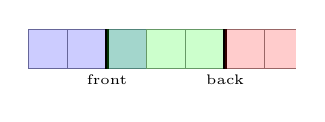
\begin{tikzpicture}[scale=0.5]
				\def\hist{2}
				\def\histext{1}
				\def\pub{3}
				\def\priv{1.8}
		
				\draw[step=1cm, gray, thin] (0, 0) grid (\hist + \pub + \priv, 1) ;
				
				\fill[blue, opacity=0.2] (0, 0) rectangle (\hist + \histext, 1) ;
				\draw[very thick] (\hist, 1) -- (\hist, 0) node[yshift=2mm, label=below:{\tiny front}] {} ;
				\fill[green, opacity=0.2] (\hist, 0) rectangle (\hist + \pub, 1) ;
				\draw[very thick] (\hist + \pub, 1) -- (\hist + \pub, 0) node[yshift=2mm, label=below:{\tiny back}] {} ;
				\fill[red, opacity=0.2] (\hist + \pub, 0) rectangle (\hist + \pub + \priv, 1) ;
			\end{tikzpicture}
	   } ;
   }
   
   \only<3->{
	   \node[align=center] (s3) [below=\height of s2] {
	   		\ding{174} emptyish \\
			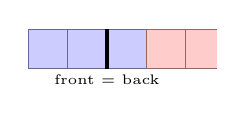
\begin{tikzpicture}[scale=0.5]
				\def\hist{2}
				\def\histext{1}
				\def\priv{2.8}
		
				\draw[step=1cm, gray, thin] (0, 0) grid (\hist + \priv, 1) ;
				
				\fill[blue, opacity=0.2] (0, 0) rectangle (\hist + \histext, 1) ;
				\draw[very thick] (\hist, 1) -- (\hist, 0) node[yshift=2mm, label=below:{\tiny front = back}] {} ;
				\fill[red, opacity=0.2] (\hist + \histext, 0) rectangle (\hist + \priv, 1) ;
			\end{tikzpicture}
	   } ;
	   \node[align=center] (s4) [below=\height of s1] {
	   	\ding{175} super empty \\
			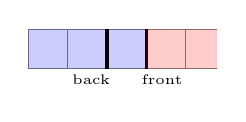
\begin{tikzpicture}[scale=0.5]
				\def\hist{2}
				\def\histext{1}
				\def\priv{2.8}
		
				\draw[step=1cm, gray, thin] (0, 0) grid (\hist + \priv, 1) ;
				
				\fill[blue, opacity=0.2] (0, 0) rectangle (\hist + \histext, 1) ;
				\draw[very thick] (\hist, 1) -- (\hist, 0) node[xshift=-2mm, yshift=2mm, label=below:{\tiny back}] {} ;
				\draw[very thick] (\hist + \histext, 1) -- (\hist + \histext, 0) node[xshift=2mm, yshift=2mm, label=below:{\tiny front}] {} ;
				\fill[red, opacity=0.2] (\hist + \histext, 0) rectangle (\hist + \priv, 1) ;
			\end{tikzpicture}
	   } ;
   }
   
   \only<2->{
	   \draw[thick, ->] (s1) to[bend left] node[above] {push} (s2) ;
	   \draw[thick, ->] (s2) to[bend left] node[below] {steal} (s1) ;
	   \draw[thick, ->] (s2) to[looseness=3, out=135, in=45] node[above] {push, pop, steal} (s2) ;
   }
   \only<4->{
	   \draw[thick, ->] (s2) to[bend left] node[right] {pop} (s3) ;
	   \draw[thick, ->] (s3) to[bend left] node[below] {pop, steal} (s4) ;
	   \draw[thick, ->] (s4) to[bend left] node[left] {pop} (s1) ;
	   \draw[thick, ->] (s1) to[bend left] node[right] {pop} (s4) ;
   }
\end{tikzpicture}
\end{frame}
\section{Prophecy variables}

\begin{frame}{Prophecy variables}
\textit{The future is ours: prophecy variables in separation logic}.

Jung, Lepigre, Parthasarathy, Rapoport, Timany, Dreyer \& Jacobs (2020).
\vfill
\[
	\begin{array}{c}
			\triple{
				\iTrue
			}{
				\texttt{NewProph}
			}{
				\lambda\ p .\,
				\exists prophs .\,
				\textcolor{blue}{\mathrm{proph}\ p\ \mathit{prophs}}
			}
		\\\\\\
			\inferrule*
				{
					\mathrm{atomic}\ e
				\\\\
					\textcolor{blue}{\mathrm{proph}\ p\ \mathit{prophs}}
				\\\\
					\weakestpre{
						e
					}{
						\begin{array}{l}
								\lambda w .\,
								\forall \mathit{prophs'} .\,
							\\
								\textcolor{red}{\mathit{prophs} = (w, v) :: \mathit{prophs'}} \iSepimp
							\\
								\textcolor{blue}{\mathrm{proph}\ p\ \mathit{prophs'}} \iSepimp
							\\
								\Phi\ w
						\end{array}
					}
				}{
					\weakestpre{
						\texttt{Resolve}\ e\ p\ v
					}{
						\Phi
					}
				}
	\end{array}
\]
\end{frame}

% ---------------------------------------------------------

\begin{frame}{Prophecy variables with memory}
\[
	\begin{array}{c}
			\triple{
				\iTrue
			}{
				\texttt{NewProph}
			}{
				\lambda\ p .\,
				\exists \textcolor{teal}{\gamma}, \mathit{prophs} .\,
				\textcolor{blue}{\mathrm{proph}\ p\ \textcolor{teal}{\gamma\ []}\ \mathit{prophs}}
			}
		\\\\\\
			\inferrule*
				{
					\mathrm{atomic}\ e
				\\\\
					\textcolor{blue}{\mathrm{proph}\ p\ \textcolor{teal}{\gamma\ \mathit{past}}\ \mathit{prophs}}
				\\\\
					\weakestpre{
						e
					}{
						\begin{array}{l}
								\lambda w .\,
								\forall \mathit{prophs'} .\,
							\\
								\textcolor{red}{\mathit{prophs} = (w, v) :: \mathit{prophs'}} \iSepimp
							\\
								\textcolor{blue}{\mathrm{proph}\ p\ \textcolor{teal}{\gamma\ (\mathit{past} \mdoubleplus [(w, v)])}\ \mathit{prophs'}} \iSepimp
							\\
								\Phi\ w
						\end{array}
					}
				}{
					\weakestpre{
						\texttt{Resolve}\ e\ p\ v
					}{
						\Phi
					}
				}
	\end{array}
\]
\end{frame}

% ---------------------------------------------------------

\begin{frame}{Prophecy variables with memory}
\begin{mathpar}
	\inferrule*[lab=ProphecyLbGet]
		{
			\mathrm{proph}\ p\ \gamma\ \mathit{past}\ \textcolor{blue}{\mathit{prophs}}
		}{
			\mathrm{proph \mathhyphen lb}\ \gamma\ \textcolor{blue}{\mathit{prophs}}
		}
	\\\\
	\inferrule*[lab=ProphecyValid]
		{
			\mathrm{proph}\ p\ \gamma\ \textcolor{red}{\mathit{past}}\ \textcolor{blue}{\mathit{prophs}_1}
		\and
			\mathrm{proph \mathhyphen lb}\ \gamma\ \textcolor{teal}{\mathit{prophs}_2}
		}{
			\exists \textcolor{purple}{\mathit{past}_1}, \textcolor{orange}{\mathit{past}_2} .\,
			{\bigwedge\left[\begin{array}{rcl}
					\textcolor{red}{\mathit{past}} = \textcolor{purple}{\mathit{past}_1} \mdoubleplus & \textcolor{orange}{\mathit{past}_2} &
				\\
					& \textcolor{orange}{\mathit{past}_2} & \mdoubleplus\, \textcolor{blue}{\mathit{prophs}_1} = \textcolor{teal}{\mathit{prophs}_2}
			\end{array}\right.}
		}
\end{mathpar}
\end{frame}

% ---------------------------------------------------------

\begin{frame}[plain, noframenumbering]
\LARGE
\begin{center}
	Thank you for your attention!
\end{center}
\end{frame}

% ---------------------------------------------------------

\appendix
\begin{frame}[fragile]{Implementation --- \texttt{chaselev\_make}}
\begin{Verbatim}[commandchars=\\\{\}]
let chaselev_make _ =
  let t = AllocN 4 () in
  t.front <- 0 ;
  t.back <- 0 ;
  t.data <- inf_array_make () ;
  \textcolor{blue}{t.prophecy <- NewProph ;}
  t
\end{Verbatim}
\end{frame}

% ---------------------------------------------------------

\begin{frame}[fragile]{Implementation --- \texttt{chaselev\_push}}
\begin{Verbatim}[commandchars=\\\{\}]
let chaselev_push t v =
  let back = !t.back in
  inf_array_set !t.data back v ;
  t.back <- back + 1
\end{Verbatim}
\end{frame}

% ---------------------------------------------------------

\begin{frame}[fragile]{Implementation --- \texttt{chaselev\_steal}}
\small
\begin{Verbatim}[commandchars=\\\{\}]
let rec chaselev_steal t =
  \textcolor{blue}{let id = NewId in}
  let front = !t.front in
  let back = !t.back in
  if front < back then (
    if Snd (
      \textcolor{blue}{Resolve} (
        CmpXchg t.front front (front + 1)
       ) \textcolor{blue}{!t.prophecy (front, id)}
    ) then (
      SOME (inf_array_get !t.data front)
    ) else (
      chaselev_steal t
    )
  ) else (
    NONE
  )
\end{Verbatim}
\end{frame}

% ---------------------------------------------------------

\begin{frame}[fragile]{Implementation --- \texttt{chaselev\_pop}}
\footnotesize
\begin{Verbatim}[commandchars=\\\{\}]
let chaselev_pop t =
  \textcolor{blue}{let id = NewId in}
  let back = !t.back - 1 in
  t.back <- back ;
  let front = !t.front in
  if back < front then (
    t.back <- front
  ) else (
    if front < back then (
      SOME (inf_array_get !t.data back)
    ) else (
      if Snd (
        \textcolor{blue}{Resolve} (
          CmpXchg t.front front (front + 1)
        ) \textcolor{blue}{!t.prophecy (front, id)}
      ) then (
        t.back <- front + 1 ;
        SOME (inf_array_get !t.data back)
      ) else (
        t.back <- front + 1 ;
        NONE
      )
    )
  )
\end{Verbatim}
\end{frame}
\begin{frame}{Infinite array}
\[
	\begin{array}{c}
			\triplePretty{
				\iTrue
			}{
				\texttt{inf\_array\_make}\ v
			}{
				\lambda\ \mathit{arr} .\ 
				\mathrm{inf \mathhyphen array \mathhyphen model}\ \mathit{arr}\ (\lambda \_ .\ v)
			}
		\\\\\\
			\atriplePretty{
				\mathit{vs}
			}{
				\mathrm{inf \mathhyphen array \mathhyphen model}\ \mathit{arr}\ \mathit{vs} \iSep
				0 \leq i
			}{
				\texttt{inf\_array\_get}\ \mathit{arr}\ i
			}{
			}{
				\mathit{vs}\ i
			}{
				\mathrm{inf \mathhyphen array \mathhyphen model}\ \mathit{arr}\ \mathit{vs}
			}
		\\\\\\
			\atriplePretty{
				\mathit{vs}
			}{
				\mathrm{inf \mathhyphen array \mathhyphen model}\ \mathit{arr}\ \mathit{vs} \iSep
				0 \leq i
			}{
				\texttt{inf\_array\_set}\ \mathit{arr}\ i\ v
			}{
			}{
				\_
			}{
				\mathrm{inf \mathhyphen array \mathhyphen model}\ \mathit{arr}\ \mathit{vs} [i \mapsto v]
			}
	\end{array}
\]
\end{frame}
\begin{frame}{Invariant}
\begin{align*}
		&\mathrm{chaselev \mathhyphen inv}\ t\ \iota
		\eqdef
	\\
		&\begin{array}{l}
				\exists \ell, \gamma, data, p \cdot \phantom{}
			\\
				\iBigsep\left[\begin{array}{l}
						t = \ell \iSep
						\mathrm{meta}\ \ell\ \gamma
					\\
						\ell\mathrm{.data} \mapsto_\square data \iSep
						\ell\mathrm{.prophecy} \mapsto_\square p
					\\
						\iInv{\iota}{\mathrm{chaselev \mathhyphen inv \mathhyphen inner}\ \ell\ \gamma\ \iota\ data\ p}
				\end{array}\right.
		\end{array}
\end{align*}
\end{frame}

% ---------------------------------------------------------

\begin{frame}{Invariant}
\begin{align*}
		&\mathrm{chaselev \mathhyphen inv \mathhyphen inner}\ \ell\ \gamma\ \iota\ data\ p
		\eqdef
	\\
		&\begin{array}{l}
				\exists front, back, hist, pub, priv, past, prophs \cdot \phantom{}
			\\
				\iBigsep\left[\begin{array}{l}
						\ell\mathrm{.front} \mapsto front \iSep
						\ell\mathrm{.back} \mapsto back
					\\
						\iGhost{\gamma\mathrm{.ctl}}{\iAuth{(back, priv)}}
					\\
						\iGhost{\gamma\mathrm{.front}}{\iAuth{front}}
					\\
						\mathrm{inf \mathhyphen array \mathhyphen model}\ data\ (hist \mdoubleplus pub)\ priv
					\\
						\iGhost{\gamma\mathrm{.pub}}{\iAuth{pub}} \iSep
						| pub | = (back - front)_+
					\\
						\mathrm{wise \mathhyphen prophet \mathhyphen model}\ p\ \gamma\mathrm{.prophet}\ past\ prophs
					\\
						\forall (front', \_) \in past \cdot front' < front
					\\
						\mathrm{chaselev \mathhyphen state}\ \gamma\ \iota\ front\ back\ hist\ pub\ prophs
				\end{array}\right.
		\end{array}
\end{align*}
\end{frame}
\begin{frame}{State}
\small
\begin{align*}
		&\mathrm{chaselev \mathhyphen state}\ \gamma\ \iota\ front\ back\ hist\ pub\ prophs
		\eqdef
	\\
		&\bigvee\left[\begin{array}{l}
				\mathrm{chaselev \mathhyphen state_1}\ \gamma\ front\ back\ hist
			\\
				\mathrm{chaselev \mathhyphen state_2}\ \gamma\ \iota\ front\ back\ hist\ pub\ prophs
			\\
				\mathrm{chaselev \mathhyphen lock}\ \gamma \iSep
				\bigvee\left[\begin{array}{l}
						\mathrm{chaselev \mathhyphen state_{3,1}}\ \gamma\ front\ back\ hist\ prophs
					\\
						\mathrm{chaselev \mathhyphen state_{3,2}}\ \gamma\ front\ back\ hist
				\end{array}\right.
		\end{array}\right.
\end{align*}
\end{frame}

% ---------------------------------------------------------

\begin{frame}{State}
\begin{align*}
		&\mathrm{chaselev \mathhyphen state_1}\ \gamma\ front\ back\ hist
		\eqdef
	\\
		&\iBigsep\left[\begin{array}{l}
				front = back
			\\
				\iGhost{\gamma\mathrm{.hist}}{\iAuth{hist}} \iSep
				| hist | = front
			\\
				\iGhost{\gamma\mathrm{.winner}}{\iAuth{-} \cdot \iFrag{-}}
		\end{array}\right.
\end{align*}
\end{frame}

% ---------------------------------------------------------

\begin{frame}{State}
\small
\begin{align*}
		&\mathrm{chaselev \mathhyphen state_2}\ \gamma\ \iota\ front\ back\ hist\ pub\ prophs
		\eqdef
	\\
		&\iBigsep\left[\begin{array}{l}
				front < back
			\\
				\iGhost{\gamma\mathrm{.hist}}{\iAuth{(hist \mdoubleplus [pub [0]])}} \iSep
				| hist | = front
			\\\\
				\begin{array}{l}
						\bold{match}\ \mathrm{filter}\ (\lambda (front', \_) \cdot front' = front)\ prophs\ \bold{with}
					\\
						|\ [] \Rightarrow
						\iGhost{\gamma\mathrm{.winner}}{\iAuth{-} \cdot \iFrag{-}}
					\\
						|\ (\_, id) :: \_ \Rightarrow
					\\
						\ \ 
						\bigvee\left[\begin{array}{l}
								\iGhost{\gamma\mathrm{.winner}}{\iAuth{-} \cdot \iFrag{-}}
							\\
								\mathrm{identifier}\ id \iSep
								\exists \Phi \cdot
								\iGhost{\gamma\mathrm{.winner}}{\iAuth{(front, \Phi)}} \iSep
								\mathrm{chaselev \mathhyphen au}\ \gamma\ \iota\ \Phi
						\end{array}\right.
				\end{array}
		\end{array}\right.
\end{align*}
\end{frame}

% ---------------------------------------------------------

\begin{frame}{State}
\small
\begin{align*}
		&\mathrm{chaselev \mathhyphen state_{3,1}}\ \gamma\ front\ back\ hist\ prophs
		\eqdef
	\\
		&\iBigsep\left[\begin{array}{l}
				front = back
			\\
				\iGhost{\gamma\mathrm{.hist}}{\iAuth{hist}} \iSep
				| hist | = front + 1
			\\\\
				\begin{array}{l}
						\bold{match}\ \mathrm{filter}\ (\lambda (front', \_) \cdot front' = front)\ prophs\ \bold{with}
					\\
						|\ [] \Rightarrow
						\iGhost{\gamma\mathrm{.winner}}{\iFrag{(front, -)}}
					\\
						|\ \_ \Rightarrow
						\exists \Phi \cdot
						\iGhost{\gamma\mathrm{.winner}}{\iAuth{(front, \Phi)}} \iSep
						\Phi (\exprSome{hist [front]})
				\end{array}
		\end{array}\right.
\end{align*}
\end{frame}

% ---------------------------------------------------------

\begin{frame}{State}
\begin{align*}
		&\mathrm{chaselev \mathhyphen state_{3,2}}\ \gamma\ front\ back\ hist
		\eqdef
	\\
		&\iBigsep\left[\begin{array}{l}
				front = back + 1
			\\
				\iGhost{\gamma\mathrm{.hist}}{\iAuth{hist}} \iSep
				| hist | = front
			\\
				\iGhost{\gamma\mathrm{.winner}}{\iAuth{-} \cdot \iFrag{-}}
		\end{array}\right.
\end{align*}
\end{frame}

% ---------------------------------------------------------

\end{document}
